% ------------------------------------------------------------------------
% ------------------------------------------------------------------------
% Modelo UFSC para Trabalhos Academicos (tese de doutorado, dissertação de
% mestrado) utilizando a classe abntex2
%
% Autor: Alisson Lopes Furlani
% 	Modificações:
%	- 27/08/2019: Alisson L. Furlani, add pacote 'glossaries' para listas
%   - 06/11/2019: Luiz-Rafael Santos, modifica para Trabalho de Conclusão de Curso
% ------------------------------------------------------------------------
% ------------------------------------------------------------------------

\documentclass[
	% -- opções da classe memoir --
	12pt,				% tamanho da fonte
	%openright,			% capítulos começam em pág ímpar (insere página vazia caso preciso)
	oneside,			% para impressão no anverso. Oposto a twoside
	a4paper,			% tamanho do papel. 
	% -- opções da classe abntex2 --
	chapter=TITLE,		% títulos de capítulos convertidos em letras maiúsculas
	section=TITLE,		% títulos de seções convertidos em letras maiúsculas
	%subsection=TITLE,	% títulos de subseções convertidos em letras maiúsculas
	%subsubsection=TITLE,% títulos de subsubseções convertidos em letras maiúsculas
	% -- opções do pacote babel --
	english,			% idioma adicional para hifenização
	%french,				% idioma adicional para hifenização
	%spanish,			% idioma adicional para hifenização
	brazil				% o último idioma é o principal do documento
	]{abntex2}

\usepackage{setup/ufscthesisA4-alf}

% ---
% Filtering and Mapping Bibliographies
% ---
% Pacotes de citações
% ---
\usepackage{csquotes}
\usepackage[backend = biber, style = abnt]{biblatex}
% FIXME Se desejar estilo numérico de citações,  comente a linha acima e descomente a linha a seguir.
% \usepackage[backend = biber, style = numeric-comp]{biblatex}

\setlength\bibitemsep{\baselineskip}
\DeclareFieldFormat{url}{Disponível~em:\addspace\url{#1}}
\NewBibliographyString{sineloco}
\NewBibliographyString{sinenomine}
\DefineBibliographyStrings{brazil}{%
	sineloco     = {\mkbibemph{S\adddot l\adddot}},
	sinenomine   = {\mkbibemph{s\adddot n\adddot}},
	andothers    = {\mkbibemph{et\addabbrvspace al\adddot}},
	in			 = {\mkbibemph{In:}}
}

\addbibresource{aftertext/references.bib} % Seus arquivos de referências

% ---
\DeclareSourcemap{
	\maps[datatype=bibtex]{
		% remove fields that are always useless
		\map{
			\step[fieldset=abstract, null]
			\step[fieldset=pagetotal, null]
		}
		% remove URLs for types that are primarily printed
%		\map{
%			\pernottype{software}
%			\pernottype{online}
%			\pernottype{report}
%			\pernottype{techreport}
%			\pernottype{standard}
%			\pernottype{manual}
%			\pernottype{misc}
%			\step[fieldset=url, null]
%			\step[fieldset=urldate, null]
%		}
		\map{
			\pertype{inproceedings}
			% remove mostly redundant conference information
			\step[fieldset=venue, null]
			\step[fieldset=eventdate, null]
			\step[fieldset=eventtitle, null]
			% do not show ISBN for proceedings
			\step[fieldset=isbn, null]
			% Citavi bug
			\step[fieldset=volume, null]
		}
	}
}
% ---

% ---
% Informações de dados para CAPA e FOLHA DE ROSTO
% ---
% FIXME Substituir 'Nome completo do autor' pelo seu nome.
\autor{Rebecca Quintino Do Ó}
% FIXME Substituir 'Título do trabalho' pelo título da trabalho.
\titulo{Projeto Final}
% FIXME Substituir 'Subtítulo (se houver)' pelo subtítulo da trabalho.  
% Caso não tenha substítulo, comente a linha a seguir.
\subtitulo{Programação C++ para Sistemas Embarcados}
% FIXME Substituir 'XXXXXX' pelo nome do seu
% orientador.
\orientador{Prof. Eduardo Augusto Bezerra}
% FIXME Se for orientado por uma mulher, comente a linha acima e descomente a linha a seguir.
% \orientador[Orientadora]{Nome da orientadora, Dra.}
% FIXME Substituir 'XXXXXX' pelo nome do seu
% coorientador. Caso não tenha coorientador, comente a linha a seguir.
\coorientador{Prof. Anderson Wedderhoff Spengler}
% FIXME Se for coorientado por uma mulher, comente a linha acima e descomente a linha a seguir.
% \coorientador[Coorientadora]{XXXXXX, Dra.}
% FIXME Substituir 'XXXXXX' pelo nome do Coordenador do 
% programa/curso.
%\coordenador{Prof. XXXXXX, Dr.}
% FIXME Se for coordenadora mulher, comente a linha acima e descomente a linha a seguir.
% \coordenador[Coordenadora]{Nome da Coordenadora, Dra.}
% FIXME Substituir '[ano da entrega]' pelo ano (ano) em que seu trabalho foi defendido.
\ano{2023}
% FIXME Substituir '[dia] de [mês] de [ano]' pela data em que ocorreu sua defesa.
\data{18 de Outubro de 2023}
% FIXME Substituir '[Cidade da defesa]' pela cidade em que ocorreu sua defesa.
\local{Florianópolis}
\instituicaosigla{UFSC}
\instituicao{Universidade Federal de Santa Catarina}
% FIXME Substituir 'Dissertação/Tese' pelo tipo de trabalho (Tese, Dissertação). 
\tipotrabalho{Projeto final}
% FIXME Substituir '[licenciado/bacharel] em [nome do título obtido]' pela grau adequado.
%\formacao{[licenciado/bacharel] em [nome do título obtido]}
% FIXME Substituir '[licenciado/bacharel]' pelo nivel adequado.
%\nivel{[licenciado/bacharel]}
% FIXME Substituir 'Curso de Graduação em [XXXXXXXX]' pela curso adequado.
\programa{Curso de Graduação em Engenharia Elétrica}
% FIXME Substituir 'Campus XXXXXX ou Centro de XXXXXX' pelo campus ou centro adequado.
\centro{Centro Tecnológico}
\preambulo
{%
\imprimirtipotrabalho~do~\imprimirprograma~do~\imprimircentro~da~\imprimirinstituicao~para~a~obtenção~do~título~de~\imprimirformacao.
}
% ---

% ---
% Configurações de aparência do PDF final
% ---
% alterando o aspecto da cor azul
\definecolor{blue}{RGB}{41,5,195}
% informações do PDF
\makeatletter
\hypersetup{
     	%pagebackref=true,
		pdftitle={\@title}, 
		pdfauthor={\@author},
    	pdfsubject={\imprimirpreambulo},
	    pdfcreator={LaTeX with abnTeX2},
		pdfkeywords={ufsc, latex, abntex2}, 
		colorlinks=true,       		% false: boxed links; true: colored links
    	linkcolor=black,%blue,          	% color of internal links
    	citecolor=black,%blue,        		% color of links to bibliography
    	filecolor=black,%magenta,      		% color of file links
		urlcolor=black,%blue,
		bookmarksdepth=4
}
\makeatother
% ---

% ---
% compila a lista de abreviaturas e siglas e a lista de símbolos
% ---

% Declaração das siglas
\siglalista{ABNT}{Associação Brasileira de Normas Técnicas}

% Declaração dos simbolos
\simbololista{C}{\ensuremath{C}}{Circunferência de um círculo}
\simbololista{pi}{\ensuremath{\pi}}{Número pi} 
\simbololista{r}{\ensuremath{r}}{Raio de um círculo}
\simbololista{A}{\ensuremath{A}}{Área de um círculo}

% compila a lista de abreviaturas e siglas e a lista de símbolos
\makenoidxglossaries 

% ---

% ---
% compila o indice
% ---
\makeindex
% ---

% ----
% Início do documento
% ----
\begin{document}

% Seleciona o idioma do documento (conforme pacotes do babel)
%\selectlanguage{english}
\selectlanguage{brazil}

% Retira espaço extra obsoleto entre as frases.
\frenchspacing 

% Espaçamento 1.5 entre linhas
\OnehalfSpacing

% Corrige justificação
%\sloppy

% ----------------------------------------------------------
% ELEMENTOS PRÉ-TEXTUAIS
% ----------------------------------------------------------
% \pretextual %a macro \pretextual é acionado automaticamente no início de \begin{document}
% ---
% Capa, folha de rosto, ficha bibliografica, errata, folha de apróvação
% Dedicatória, agradecimentos, epígrafe, resumos, listas
% ---
% ---
% Capa
% ---
\imprimircapa
% ---

% ---
% Folha de rosto
% (o * indica que haverá a ficha bibliográfica)
% ---
\imprimirfolhaderosto*
% ---

% ---
% Inserir a ficha bibliografica
% ---
% http://ficha.bu.ufsc.br/
\begin{fichacatalografica}
	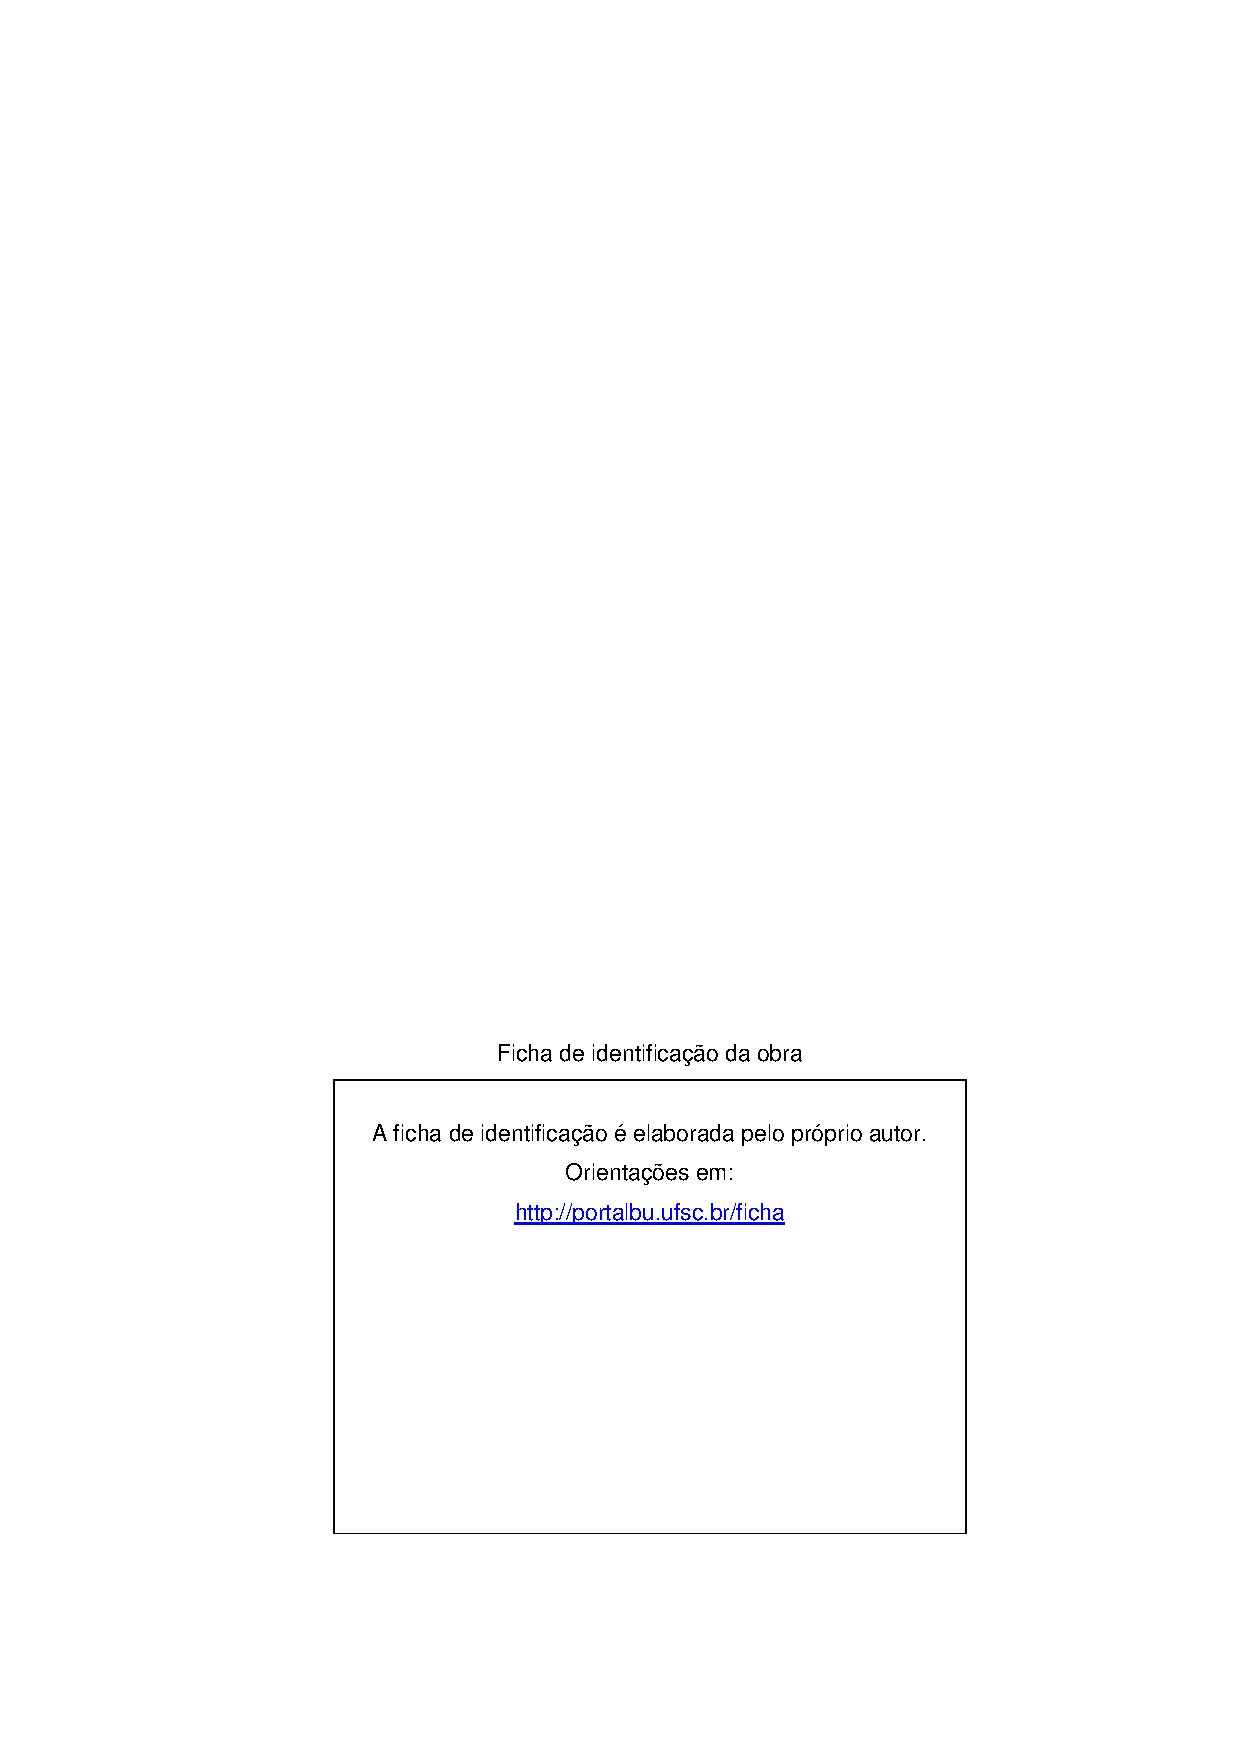
\includepdf{beforetext/Ficha_Catalografica.pdf}
\end{fichacatalografica}
% ---

% ---
% Inserir folha de aprovação
% ---
% \begin{folhadeaprovacao}
% 	\OnehalfSpacing
% 	\centering
% 	\imprimirautor\\%
% 	\vspace*{10pt}		
% 	\textbf{\imprimirtitulo}%
% 	\ifnotempty{\imprimirsubtitulo}{:~\imprimirsubtitulo}\\%
% 			\vspace*{31.5pt}%3\baselineskip
% 	\vspace*{\baselineskip}
% 	\begin{minipage}{\textwidth}
% 	~do~\imprimirprograma~do~\imprimircentro~da~\imprimirinstituicao~para~a~obtenção~do~título~de~\imprimirformacao.
% 	Este~\imprimirtipotrabalho~foi julgado adequado para obtenção do Título de “\imprimirformacao” e aprovado em sua forma final pelo~\imprimirprograma. \\
% 		\vspace*{\baselineskip}
% 	\imprimirlocal, \imprimirdata. \\
% 	\vspace*{2\baselineskip}
% 	\assinatura{\OnehalfSpacing\imprimircoordenador \\ \imprimircoordenadorRotulo~do Curso}
% 	\vspace*{2\baselineskip}
% 	\textbf{Banca Examinadora:} \\
% 	\vspace*{\baselineskip}
% 	\assinatura{\OnehalfSpacing\imprimirorientador \\ \imprimirorientadorRotulo}
% 	%\end{minipage}%
% 	\vspace*{\baselineskip}
% 	\assinatura{Prof.(a) xxxx, Dr(a).\\
% 	Avaliador(a) \\
% 	Instituição xxxx}

% 	\vspace*{\baselineskip}
% 	\assinatura{Prof.(a) xxxx, Dr(a).\\
% 	Avaliador(a) \\
% 	Instituição xxxx}


% \end{folhadeaprovacao}
% ---

% ---
% Dedicatória
% ---
% \begin{dedicatoria}
% 	\vspace*{\fill}
% 	\noindent
% 	\begin{adjustwidth*}{}{5.5cm}     
% 		Este trabalho é dedicado aos meus colegas de classe e aos meus queridos pais.
% 	\end{adjustwidth*}
% \end{dedicatoria}
% ---

% ---
% Agradecimentos
% ---
% \begin{agradecimentos}
% 	Inserir os agradecimentos aos colaboradores à execução do trabalho. 
	
% 	Xxxxxxxxxxxxxxxxxxxxxxxxxxxxxxxxxxxxxxxxxxxxxxxxxxxxxxxxxxxxxxxxxxxxxx. 
% \end{agradecimentos}
% ---

% ---
% Epígrafe
% ---
% \begin{epigrafe}
% 	\vspace*{\fill}
% 	\begin{flushright}
% 		\textit{``Texto da Epígrafe.\\
% 			Citação relativa ao tema do trabalho.\\
% 			É opcional. A epígrafe pode também aparecer\\
% 			na abertura de cada seção ou capítulo.\\
% 			Deve ser elaborada de acordo com a NBR 10520.''\\
% 			(Autor da epígrafe, ano)}
% 	\end{flushright}
% \end{epigrafe}
% ---

% ---
% RESUMOS
% ---

% resumo em português
\setlength{\absparsep}{18pt} % ajusta o espaçamento dos parágrafos do resumo
\begin{resumo}
	\SingleSpacing
	No resumo são ressaltados o objetivo da pesquisa, o método utilizado, as discussões e os resultados com destaque apenas para os pontos principais. O resumo deve ser significativo, composto de uma sequência de frases concisas, afirmativas, e não de uma enumeração de tópicos. Não deve conter citações. Deve usar o verbo na voz ativa e na terceira pessoa do singular. O texto do resumo deve ser digitado, em um único bloco, sem espaço de parágrafo. O espaçamento entre linhas é simples e o tamanho da fonte é 12. Abaixo do resumo, informar as palavras-chave (palavras ou expressões significativas retiradas do texto) ou, termos retirados de thesaurus da área. Deve conter de 150 a 500 palavras. O resumo é elaborado de acordo com a NBR 6028.
	
	\textbf{Palavras-chave}: Palavra-chave 1. Palavra-chave 2. Palavra-chave 3.
\end{resumo}

% resumo em inglês
\begin{resumo}[Abstract]
	\SingleSpacing
	\begin{otherlanguage*}{english}
		Resumo traduzido para outros idiomas, neste caso, inglês. Segue o formato do resumo feito na língua vernácula. As palavras-chave traduzidas, versão em língua estrangeira, são colocadas abaixo do texto precedidas pela expressão “Keywords”, separadas por ponto.
		
		\textbf{Keywords}: Keyword 1. Keyword 2. Keyword 3.
	\end{otherlanguage*}
\end{resumo}

%% resumo em francês 
%\begin{resumo}[Résumé]
% \begin{otherlanguage*}{french}
%    Il s'agit d'un résumé en français.
% 
%   \textbf{Mots-clés}: latex. abntex. publication de textes.
% \end{otherlanguage*}
%\end{resumo}
%
%% resumo em espanhol
%\begin{resumo}[Resumen]
% \begin{otherlanguage*}{spanish}
%   Este es el resumen en español.
%  
%   \textbf{Palabras clave}: latex. abntex. publicación de textos.
% \end{otherlanguage*}
%\end{resumo}
%% ---

{%hidelinks
	\hypersetup{hidelinks}
	% ---
	% inserir lista de ilustrações
	% ---
	\pdfbookmark[0]{\listfigurename}{lof}
	\listoffigures*
	\cleardoublepage
	% ---
	
	% ---
	% inserir lista de quadros
	% ---
	\pdfbookmark[0]{\listofquadrosname}{loq}
	\listofquadros*
	\cleardoublepage
	% ---
	
	% ---
	% inserir lista de tabelas
	% ---
	\pdfbookmark[0]{\listtablename}{lot}
	\listoftables*
	\cleardoublepage
	% ---
	
	% ---
	% inserir lista de abreviaturas e siglas (devem ser declarados no preambulo)
	% ---
	\imprimirlistadesiglas
	% ---
	
	% ---
	% inserir lista de símbolos (devem ser declarados no preambulo)
	% ---
	\imprimirlistadesimbolos
	% ---
	
	% ---
	% inserir o sumario
	% ---
	\pdfbookmark[0]{\contentsname}{toc}
	\tableofcontents*
	\cleardoublepage
	
}%hidelinks
% ---
% ---

% ----------------------------------------------------------
% ELEMENTOS TEXTUAIS
% ----------------------------------------------------------
\textual

% ---
% 1 - Introdução
% ---
% ----------------------------------------------------------
\chapter{Introdução}
% ----------------------------------------------------------

% ----------------------------------------------------------
\section{Recomendações de uso}
% ----------------------------------------------------------


% ----------------------------------------------------------
\section{Objetivos}
% ----------------------------------------------------------


% % ----------------------------------------------------------
% \subsection{Objetivo Geral}
% % ----------------------------------------------------------

% % ----------------------------------------------------------
% \subsection{Objetivos Específicos}
% % ----------------------------------------------------------


% ---

% ---
% 2 - Capítulo 2
% ---
% ----------------------------------------------------------
\chapter{Desenvolvimento}\label{cap:desenvolvimento}
% ----------------------------------------------------------

% ----------------------------------------------------------
\section{Exposição do tema ou matéria}
% ----------------------------------------------------------


% ----------------------------------------------------------
\section{Orçamento}
% ----------------------------------------------------------

\begin{table}[htb]
	\ABNTEXfontereduzida
	\caption{\label{tab:orçamento}Orçamento do projeto}
    \centering
	\begin{tabular}{lccc} 
		\toprule
		\textbf{Item} & \textbf{Valor unitário} & \textbf{Quantidade} & \textbf{Total}\\
		Kit Módulo Leitor Rfid Mfrc522 Mifare & R\$ 17.95 & 1 & R\$ 17.95  \\
		Protoboard 400 Pontos                 & R\$ 9.40  & 1 & R\$ 9.40  \\
		Módulo WiFi ESP32 Bluetooth           & R\$ 58.80 & 1 & R\$ 58.80  \\
		\bottomrule
	\end{tabular}
\end{table}
% ---

% ---
% 3 - Capítulo 3
% ---
% ----------------------------------------------------------
\chapter{Conclusão}
% ----------------------------------------------------------

As conclusões devem responder às questões da pesquisa, em relação aos objetivos e às hipóteses. Devem ser breves, podendo apresentar recomendações e sugestões para trabalhos futuros.
% ---

% ---
% 4 - Conclusão
% ---
%\phantompart
\include{chapters/4-chapter}
% ---

% ----------------------------------------------------------
% ELEMENTOS PÓS-TEXTUAIS
% ----------------------------------------------------------
\postextual
% ----------------------------------------------------------

% ----------------------------------------------------------
% Referências bibliográficas
% ----------------------------------------------------------
\begingroup
    \SingleSpacing\printbibliography[title=REFERÊNCIAS]
\endgroup

% ----------------------------------------------------------
% Glossário
% ----------------------------------------------------------
%
% Consulte o manual da classe abntex2 para orientações sobre o glossário.
%
%\glossary

% ----------------------------------------------------------
% Apêndices
% ----------------------------------------------------------

% ---
% Inicia os apêndices
% ---
\begin{apendicesenv}
%	\partapendices* 
	% ----------------------------------------------------------
\chapter{Descrição}
% ----------------------------------------------------------

Textos elaborados pelo autor, a fim de completar a sua argumentação. Deve ser precedido da palavra APÊNDICE, identificada por letras maiúsculas consecutivas, travessão e pelo respectivo título. Utilizam-se letras maiúsculas dobradas quando esgotadas as letras do alfabeto. 

\begin{quadro}[htb]
	\centering
	\caption{\label{qua:Quadro_2}Modelo A.}	
\begin{tabular}{|l|l|}
\hline
xxxx              & yyyyyyyyyyyyyyy    \\
\hline
xxxx              & yyyyyyyyyyyyyyy    \\
\hline
xxxx              & yyyyyyyyyyyyyyy    \\
\hline
xxxx              & yyyyyyyyyyyyyyy    \\
\hline
xxxx              & yyyyyyyyyyyyyyy    \\
\hline
xxxx              & yyyyyyyyyyyyyyy    \\
\hline
xxxx              & yyyyyyyyyyyyyyy    \\
\hline
rrrrrrrrrrrrrrrrr & eeeeeeeeeeeeeeeee  \\
\hline
xxxx              & yyyyyyyyyyyyyyy    \\
\hline
xxxx              & yyyyyyyyyyyyyyy    \\
\hline
rrrrrrrrrrrrrrrrr & eeeeeeeeeeeeeeeee  \\
\hline
xxxx              & yyyyyyyyyyyyyyy    \\
\hline
                  & ttttttttttttttttt  \\
\hline
rrrrrrrrrrrrrrrrr & eeeeeeeeeeeeeeeee  \\
\hline
ttttttttttttt     &                    \\
\hline
rrrrrrrrrrrrrrrrr & eeeeeeeeeeeeeeeee  \\
\hline
rrrrrrrrrrrrrrrrr & eeeeeeeeeeeeeeeee  \\
\hline
                  & gggggggggggggggggg \\
\hline
rrrrrrrrrrrrrrrrr & eeeeeeeeeeeeeeeee  \\
\hline
rrrrrrrrrrrrrrrrr & eeeeeeeeeeeeeeeee  \\
\hline
rrrrrrrrrrrrrrrrr & eeeeeeeeeeeeeeeee  \\
\hline
rrrrrrrrrrrrrrrrr & eeeeeeeeeeeeeeeee  \\
\hline
\end{tabular}
\fonte{Elaborada pelo autor (2016).}
\end{quadro}
\end{apendicesenv}
% ---


% ----------------------------------------------------------
% Anexos
% ----------------------------------------------------------

% ---
% Inicia os anexos
% ---
\begin{anexosenv}
%	\partanexos*
	% ----------------------------------------------------------
\chapter{Descrição}
% ----------------------------------------------------------

São documentos não elaborados pelo autor que servem como fundamentação (mapas, leis, estatutos). Deve ser precedido da palavra ANEXO, identificada por letras maiúsculas consecutivas, travessão e pelo respectivo título. Utilizam-se letras maiúsculas dobradas quando esgotadas as letras do alfabeto. 

\end{anexosenv}

%---------------------------------------------------------------------
% INDICE REMISSIVO
%---------------------------------------------------------------------
%\phantompart
%\printindex
%---------------------------------------------------------------------

\end{document}
